\chapter{Destination Choice}
\label{ch:destinationchoice}
% ##################################################################################################################
\hfill \textbf{Author:} Andreas Horni

\begin{center} \includegraphics[width=0.5\textwidth, angle=0]{extending/figures/dc/zhLeisure.pdf} \end{center}

% ##################################################################################################################
\section{Basic Concept}
The MATSim destination choice problem represents an optimization problem, where every agent searches for his optimal destination according to an objective function, which is based on discrete choice theory described in length by \citet[][]{Horni_PhDThesis_2013, HorniEtAl_unpub_TRB_2012}. The framework provides a problem-tailored heuristic search algorithm and an adaptable objective function containing a systematic and a random part representing unobserved heterogeneity. Due to the iterative mechanism of MATSim choices are performed based on quenched and not annealed randomness as detailed in the next section. 

The destination choice module can be configured to consider not only competition for the road infrastructure but also the activities infrastructure (for example at shopping malls' parking lots) \citep[][]{HorniEtAl_TRR_2009}.

% ##################################################################################################################
\section{Running Destination Choice}
The contribution destination choice is applied by adapting the configuration file strategy module,
%
\begin{lstlisting}
<module name="strategy" > 
    <param name="ModuleProbability_1" value="0.x" /> 
    <param name="Module_1" value="locationchoice" /> 
    [...]
</module>
\end{lstlisting}
%
by defining its parameters in the configuration file destination choice section, 
%
\begin{lstlisting}
<module name="locationchoice" > 
    <param name="param0" value="value0" /> 
    [...]
</module>
\end{lstlisting}
%
and by running the special controler \lstinline|DCControler| residing in the package \lstinline|org.matsim.contrib.locationchoice|

% ##################################################################################################################
\section{Application of the Module}
The destination choice module has been successfully applied for the Z�rich scenario (Section \ref{sec:scenario.zh})) as reported in \citet[][p.99]{Horni_PhDThesis_2013}, for the Tel Aviv model (see Section \ref{sec:scenario.telaviv}) and for the MATSim 2030 project. Figures \ref{fig:zhLEGO} and \ref{fig:countsLEGO} show that by means of scaling of the error terms distance distributions can be nicely fitted and that thereby the error in count data is decreased.

\createfigure%
{Error Term Runs for the Zurich scenario}%
{Error Term Runs for the Zurich scenario}%
{\label{fig:zhLEGO}}%
{%
  \createsubfigure%
  {Shopping trips}%
	{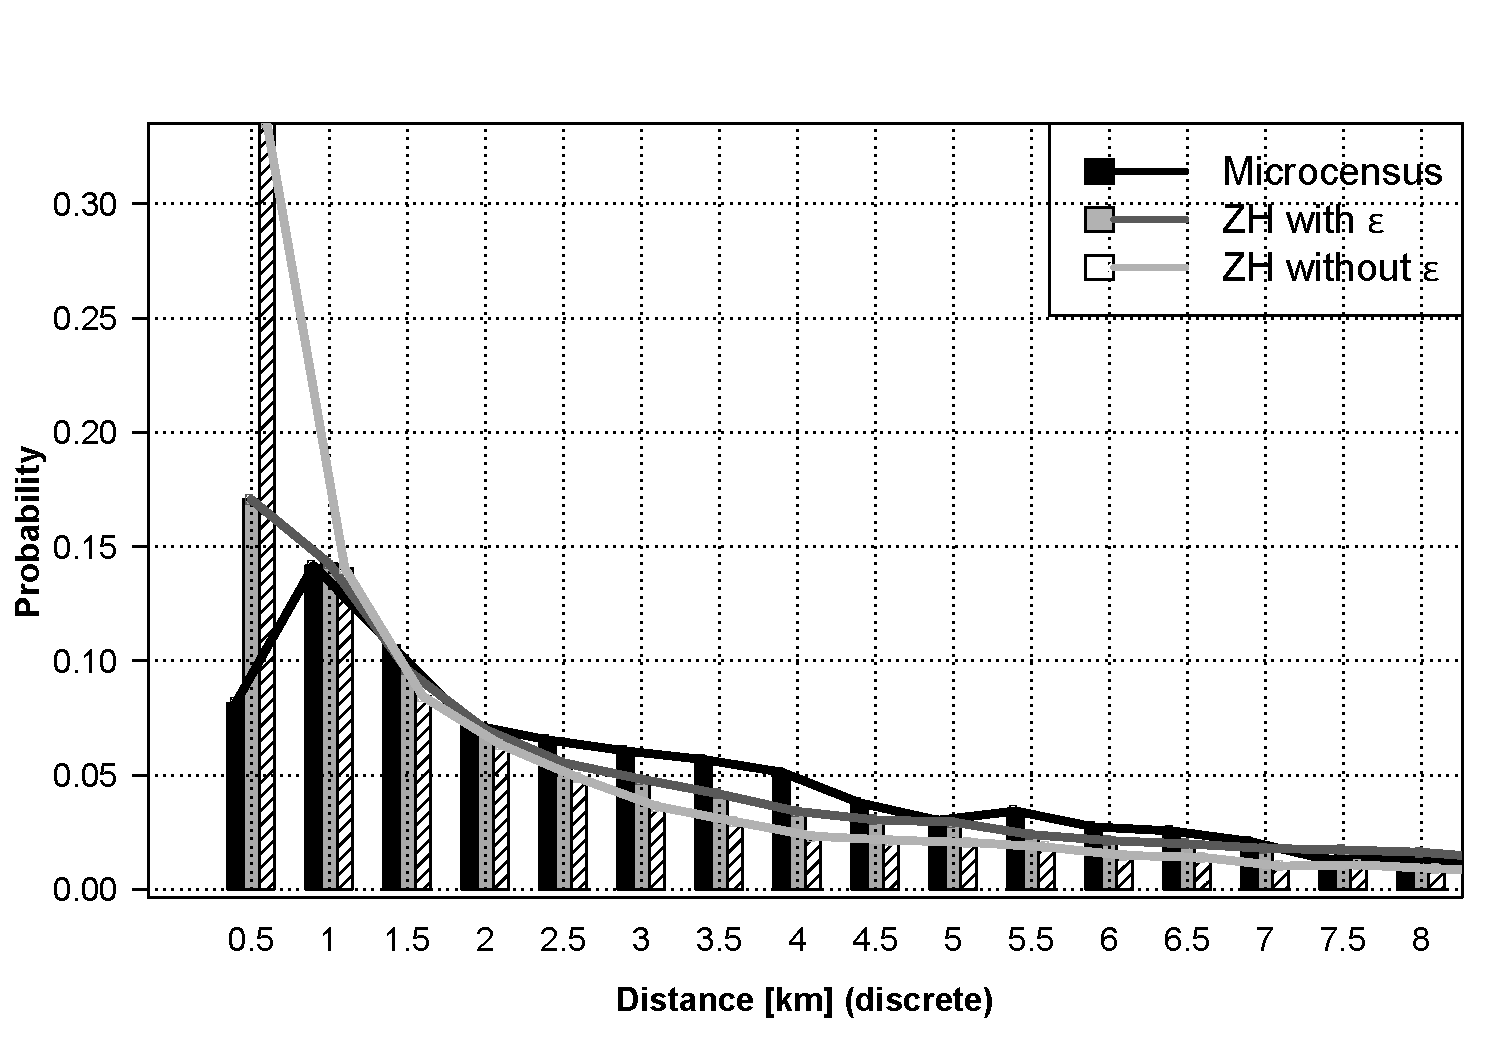
\includegraphics[width=0.99\textwidth,angle=0]{extending/figures/dc/zhShopping.pdf}}%
  {\label{fig:zhShopping}}%
  {}%
   \createsubfigure%
  {Leisure trips}%
  {\includegraphics[width=0.99\textwidth,angle=0]{extending/figures/dc//zhLeisure.pdf}}%
  {\label{fig:zhLeisure}}%
  {}%
}%
{}

\createfigure%
{Daily traffic volumes for 123 links compared to traffic counts}%
{Daily traffic volumes for 123 links compared to traffic counts. Per link $k$ the relative error is used, i.e, $(vol_{simulated,k}-vol_{counted,k}) / vol_{counted,k}$.}%
{\label{fig:countsLEGO}}%
{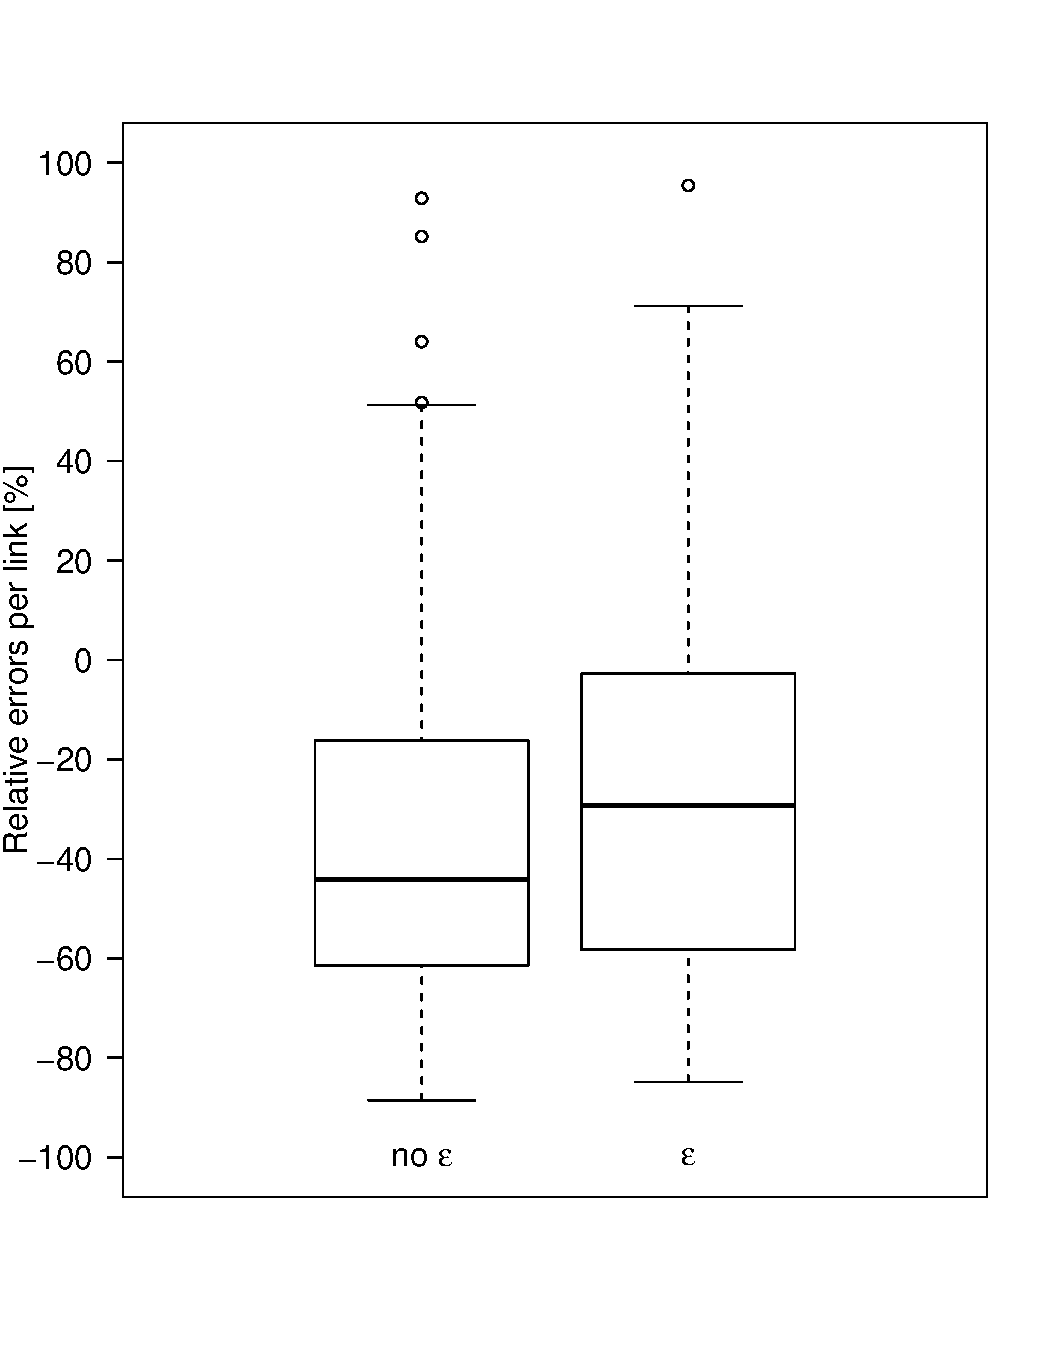
\includegraphics[width=0.8\textwidth, angle=0]{extending/figures/dc/zhCounts.pdf}}%
{}

% ##################################################################################################################
\section{Key Problems in Developing the Module}
Key problems of integrating destination choice into MATSim span behavioral and algorithmic issues. On the behavioral side, the specification of choice sets for model estimation is an unsolved problem to date. On the algorithmic side, as mentioned above, destination choice is in principle an ordinary optimization problem. However, as the agents interact and as the choices are embedded in a highly dynamic context, the problem becomes complex, even more as the targeted scenarios are usually large-scale. Thus, as is common for real-world optimization problems, solutions have to be based on problem-tailored heuristics \citep[][]{MichalewiczFogel_2004}. Important components of the MATSim destination choice are the construction of a limited search space and of the succeeding evaluation of this search space's elements. The main component however, is a mechanism to generate consistent random draws over the iterations necessary to include the objective function's error terms. This mechanisms is also applicable for other choice dimensions.

% --------------------------------------------------------------------
\subsection{Quenched Randomness}
In random utility theory, decision makers are assumed to be rational utility maximizers, where the utility is dependent on the characteristics of the alternatives, the choice maker itself and the choice situation. Besides these deterministic components, unobserved heterogeneity must be added by random error terms, often denoted $\epsilon$. Due to these random error terms choices are quantified by probabilities dependent, for the logit model for example as $p_{jli} = \exp(V_{jli}) / \sum_q exp(V_{jqi})$, where $V_{jli}$ is person $j$'s systematic utility of alternative $l$ for activity $i$, which is divided by all remaining choice set's alternatives $q$. When drawing from the distribution specified by $p_{jli}$ for a population, the aggregate choices are reproduced. This is basically also true, when applied in iterative frameworks. However, iterative frameworks are usually associated with some kind of learning or relaxation mechanism. This mechanism is heavily distorted by repeatedly and randomly drawing from $p_{jli}$ in every iteration. In this case the $epsilon_{jli}$ fluctuate from iteration to iteration, which is disastrous for the algorithm's convergence and behaviorally implausible.

Instead, the random error terms $\epsilon_{jl}$ need to remain fixed from iteration to iteration. The optimization is then performed as a deterministic search based on the resulting utilities $U_{jli}$, i.e., an alternative $l$ for person $j$ and activity $i$ is selected as 
\[ 
\underset{l \in choice\: set}{\operatorname{argmax}} U_{jli} \,.
\] 
This includes, via the systematic part $V_{jli}$, the disutility of traveling to destination $l$ for activity~$i$.

As stated above, the random error terms need to remain the same over the iterations. In physics, this approach would be called ``quenched'' randomness; all randomness is computed initially and then attached to particles or destinations, rather than instantaneously generating it, which would be called ``annealed'' randomness. Two natural approaches for implementing quenched randomness are as follows:
\begin{itemize}
\item[(a)] Freezing the applied \emph{global} sequence of random numbers, meaning that a Monte Carlo method with the same random seed is used before and after the introduction of a policy measure and over the course of iterations. Thus, the error terms should come out the same way \emph{before} and \emph{after} the introduction of the policy measure. Differences in the outcome can thus be directly attributed to the policy measure. 
\item[(b)] Computing and storing a separate $\epsilon_{jli}$ for every combination of person $j$, alternative~$l$ and activity $i$.
\end{itemize}
 
Both strategies have flaws. Approach (a) is only an option if one is certain about every single aspect of the computational code. Importantly, one additional random number, drawn in one run but not in the other, completely destroys the ``quench'' for all decisions computed later in the program. Consistency is thus hard to achieve, especially in parallel or even distributed computing environments; according to personal communication a substantial machinery is necessary ensuring consistent choices. In a modular environment, as in MATSim, designed for external plugging-in of users' own modules---possibly drawing their own random numbers---the danger of destroying the quench is prohibitively high and thus approach (a) is impractical.

Approach (b) is certainly more robust. However, for large numbers of decision makers and/or alternatives, storing error terms is difficult. For destination choice, one quickly has $10^6$ decision makers and $10^6$ alternatives, resulting in $4 \times 10^{12} \hbox{Byte} = 4 \hbox{TByte}$ of storage space.

One may argue that this should not be a problem, since a normal person will rarely consider more than the order of a hundred alternatives in their choice set, reducing the computational problem. Aside from the necessity of storing every decision maker's choice set, this converts the computational problem into a conceptual one, since a good method to generate choice sets then needs to be found. With more conceptual progress, this may eventually be an option, but at this point, a conceptually simpler approach is preferred.

The developed solution below is generally applicable in econometric microsimulators. The same \emph{stable} error term can be \emph{re-}calculated on the fly by using stable random seeds $s_{jli} = g(k_j, k_l, k_i)$, where are uniformly distributed random numbers associated with $j$, $l$, and $i$. That is, for each person $j$ a random number $k_j$ is generated and stored, and the same is done with each destination $l$. The value for the activity $i$ can be derived from its index in the plan possibly combined with the person's value $k_j$. This reduces the storage space dramatically from $\bar{ni} \times nj \times nl$ to $\bar{ni}(nj + nl)$, where $nj$ is the number of persons or agents and $n_l$ is the number of destinations and $\bar{ni}$ is the average number of discretionary activities in an agent's plan. This means that storage space is reduced to approx. $2 \times 4 \times 10^{6} \hbox{Byte} = 8 \hbox{MByte}$, which can be easily stored even on any modern machine.

The distribution of these seeds is essentially irrelevant; any error term distribution can be generated from any basic seed distribution. 
In the current version $g(k_j, k_l, k_i) = (k_j + k_l + k_i) \times v_{max}$ is used. $v_{max}$ is the maximum (long) number that can be handled by the specific machine.

To evaluate utility for a person $j$ visiting the destination $l$ for activity $i$ a sequence of Gumbel-distributed random numbers $seq_{jli}$ is generated on the fly for every person-alternative-activity combination using the seed $s_{jli}$. Some random number generators have problems in the initial phase of drawing, e.g., the first couple of random numbers are correlated or do never cover the complete probability space. As in our procedure the random number generator is constantly re-initialized, for these technical reasons, the error term $\epsilon_{jli}$ is derived not from the first element but from the $m^{th}$ element of the sequence $seq_{jli}[m]$. Here, $m$ is set to 10. This procedure is valid as the set of all  $m^{th}$ elements of all different sequences is also a pseudo-random sequence following the same distribution as the sequences $seq_{jli}$; clearly, \emph{true} random number generators relying on physical phenomena, such as hardware temperature, are not applicable. 

% ------------------------------------------
\subsection{Search Space Construction and Evaluation:}
MATSim destination choice is based on best-response rather than random mutation, i.e., in every iteration the currently best alternative is chosen. This works as long as the inter-iteration changes are small, which is usually given by the relatively small share of agents who re-plan. The best-response approach is adopted due to the usually huge number of alternatives in combination with the search space characteristics. As the discrete search landscape is characterized by random noise because error terms are not (or only locally) spatially correlated (see Figure \ref{fig:landscape0}). For such problems---as opposed to continuous landscapes (see Figure \ref{fig:landscape1})---efficient search methods, such as local search methods, generally do not work.

% ---------------------------------
\createfigure%
{Search space}%
{Search space: The search algorithm is required to be able to handle correlated but also uncorrelated error terms as given by the MNL model. Local search methods, such as hill-climbing algorithms are only able to handle continuous search spaces, thus, for situation (a) a best-response global search algorithm is required.}%
{\label{fig:landscape}}%
{%
  \createsubfigure%
  {Uncorrelated error terms}%
  {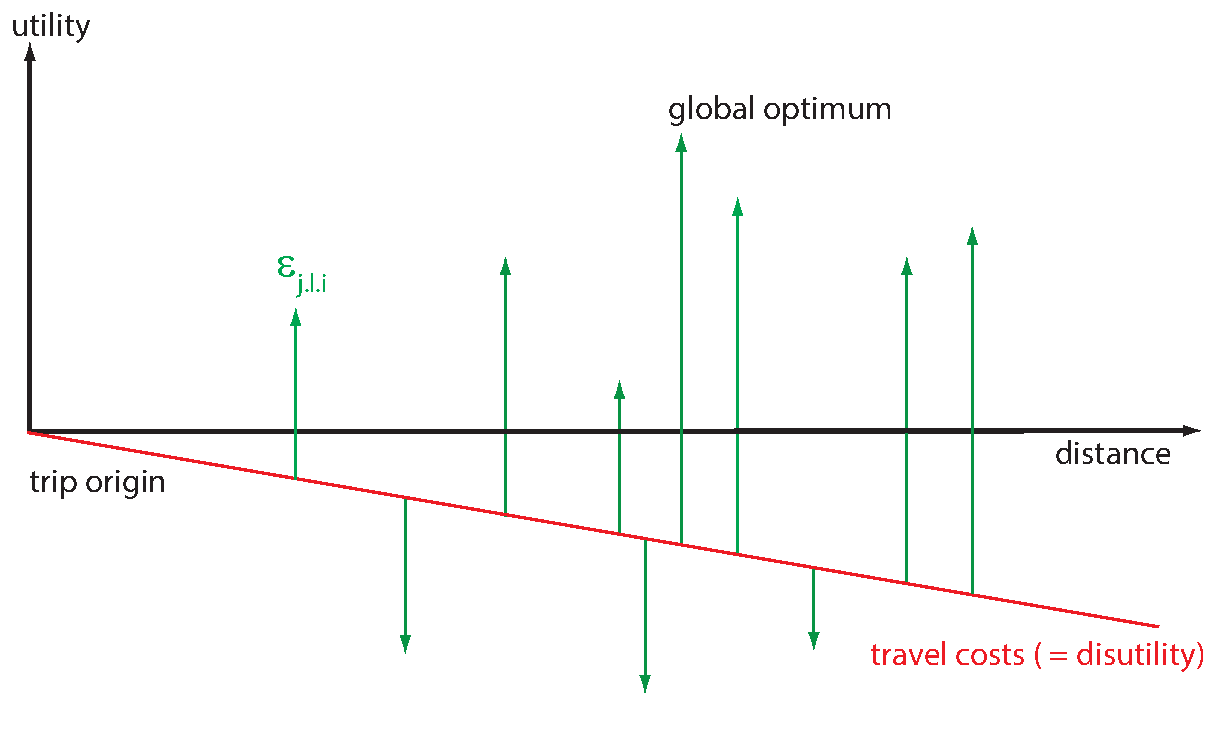
\includegraphics[width=0.8\textwidth,angle=0]{extending/figures/dc/landscape1.pdf}}%
  {\label{fig:landscape0}}%
  {}%
  \createsubfigure%
  {Spatially correlated error terms}%
	{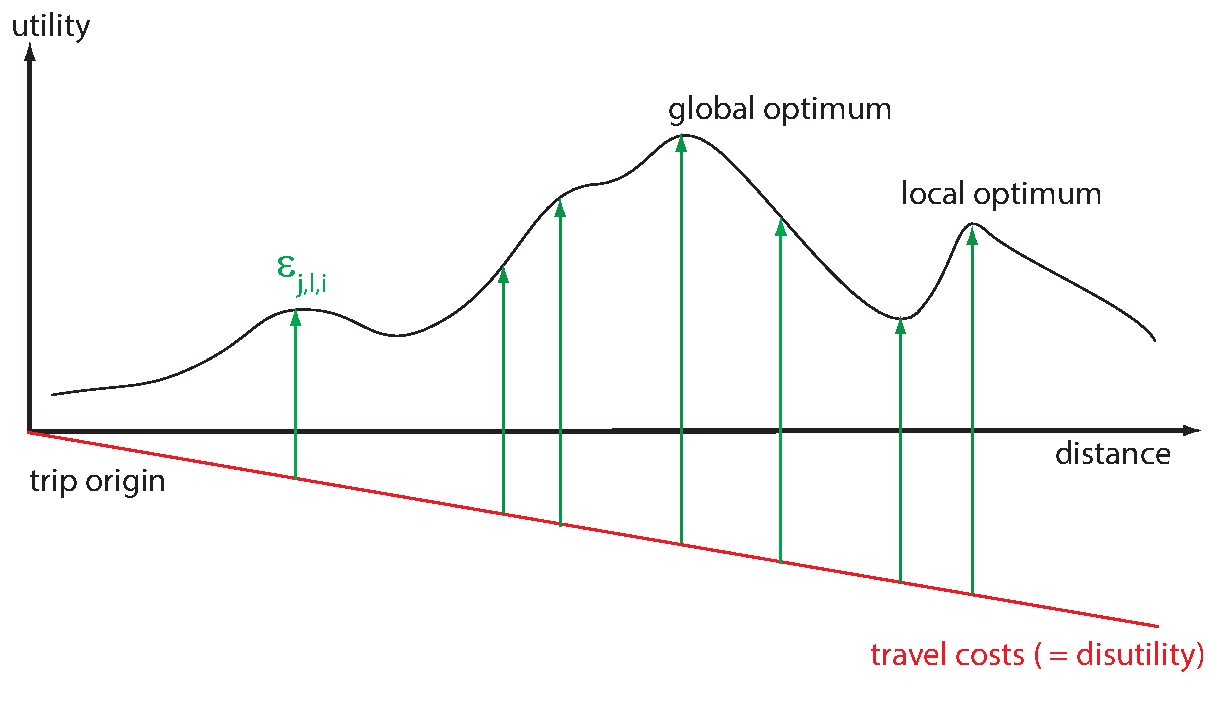
\includegraphics[width=0.8\textwidth,angle=0]{extending/figures/dc/landscape0.pdf}}%
  {\label{fig:landscape1}}%
  {}%
}%
{}

% ---------------------------------
On the search for the best choice, the large number of alternatives---prohibiting exhaustive search---is restrained as follows (for the detailed derivation see \citet[][p.51 ff.]{Horni_PhDThesis_2013}). It is assumed that travel costs are always negative, and that a person drops activities with negative net utility. Then the maximum potential travel effort a person is willing to invest is constrained by the maximum error term per person and activity. This approach is promising, as very large values for Gumbel-distributed are rare, meaning that a huge space must be searched for only a few persons. 

This reduction of the search space saves a lot of computation time, however, it is still infeasible and further speed-ups are necessary. Most computation time is due to calculation of travel times, i.e.,\ due to routing, for evaluation of the alternatives in the search space. To reduce these huge routing costs, the Dijkstra is not only applied forward---providing one-to-all travel times--but also \emph{backwards} using an average estimated arrival time as initial time. This is an approximation, and thus a \emph{probabilistic} best response is applied, justified by the natural assumption that, during the course of the iterations, the probabilistic choice probably reduces, or even compensates, the errors incurred by approximating travel times. 

With this procedure, the required computational effort is dramatically reduced, allowing application of destination choice to large-scale scenarios.

% ------------------------------------------
\subsection{Destination Choice Set Specification:}
While choice set specification is natural for choices with few alternatives, in contrast, for problems with a large universal choice set, usually present for spatial choices, such as destination or route choice, specifying individual choice sets becomes a challenging computational and even more behavioral issue (see e.g., \citet[][]{PagliaraTimmermans_TransLett_2009, Thill_PHG_1992, Schuessler_PhDThesis_2010, FrejingerEtAl_TransResB_2009}. Estimated parameters are sensitive to choice sets, and, at the same time, no established choice set definition procedure exists for spatial problems. This means that choice sets and, hence, estimation results are highly dependent on the modeler, which is an exogeneity problem, structurally similar to the well-known ``Modifiable Areal Unit Problem'' (MAUP), where results are dependent on modeler's zoning specification.

A prominent extension of the standard discrete choice modeling approach to treat this problem is formed by stochastic choice set models, founded by \citet[][]{Manski_TD_1977, BurnettKPHanson_TRR_1979, BurnettKP_UG_1980}, which integrates the choice set formation step into the estimation procedure by jointly estimating selection of a choice set and the choice of a particular alternative of this choice set \citep[][]{KaplanEtAl_TRB_2009, PagliaraTimmermans_TransLett_2009, Manski_TD_1977, Swait_TransResPartB_2001, HorowitzLouviere_IJRM_1995, BenAkivaBoccara_IJRM_1995, SwaitBenAkiva_TransResPartB_1987, Swait_TransResPartB_2001, MartinezEtAl_TransResPartB_2009, CascettaPapola_TransResPartA_2009, BierlaireEtAl_2_STRC_2009, ScroginEtAl_TechRep_UCF_2004, ManraiAndrews_EJOR_1998, Ansah_TransRes_1977}. Probabilistic choice set formation is conceptually appealing as choice sets are, in principle, not restrained a priori by exogenous criteria as in standard choice set specification. However, the procedure is in general associated with combinatorial complexity, making it computationally intractable. As a consequence, the practical approaches also require mechanisms to reduce the complexity of the choice set specification problem (see e.g., \citet[][p.11]{BenAkivaBoccara_IJRM_1995}). \citet[][]{ZhengJieGuo_TRB_2008}, for example, make the moderate assumption of continuous store choice sets (i.e., sets without ``holes'') around the trip origin, while the random-constraints model of \citet[][]{BenAkivaBoccara_IJRM_1995} exploits additional information on alternatives' availability for individuals.

Concluding, the destination choice set specification problem is still unsolved, meaning that the estimated models can only be fully consistently applied for the region, where the model was estimated. For MATSim, first destination choice model estimation efforts are reported in \citet[][Chapter 5]{Horni_PhDThesis_2013}.

% ##################################################################################################################
\section{The Module in the MATSim Context}
The destination choice module explicitly incorporates unobserved heterogeneity through random error terms. The standard MATSim utility function, however, does not contain error terms. The randomness measured in empirical data is included implicitly and in an uncontrolled way through the stochasticity of the simulation process. For destination choice, this has led to a dramatic underestimation of total travel demand making inclusion of unobserved heterogeneity inevitable. In the future, it should be researched if the standard utility function might also profit from the innovations of the destination choice module.

As detailed in Section \ref{sec:bestResponseOrRandom} MATSim replanning offers different strategies to adapt plans ranging from random mutation to approximate suggestions, to best response answers. Destination choice is based on best response due to the sheer size of the alternatives set. 

As discussed in Chapter \ref{ch:scoring}, final goal is the implementation of an estimated utility function. At the moment, however, the standard MATSim scoring is still based on the Charypar-Nagel function and extended ad hoc by few attributes. This is also true for the destination choice module. Thus, calibration---instead of estimation---of the utility function is performed such that measured travel distances are matched. Calibration is performed by scaling the error terms. 

Although, the destination choice utility function is based on the discrete choice framework, some conceptual differences to the common application of discrete choice models exist. As shown above, there is no drawing from discrete choice models but maximization of an iteration stable utility function. In relation to that, the set of alternatives is not necessarily limited a priori and, thus, has the notion of a search space and not of a choice set.

% ##################################################################################################################
\section{Lessons Learned}
Two interesting lessons have been learning while developing the destination choice module. The first is a lesson of interdependence of preferences and space and,  thus, the necessity to evaluate them in combination. When looking at distance distributions (e.g., Figure \ref{fig:zhLEGO}) one might think that the functional form directly represents the preferences. This is not necessarily the case. In our simulations, it is the result of a \emph{linear} travel disutility applied in geographic space, where the number of opportunities increases with the square of the radius, in other words, with the travel distance. A similar emergent effect is present when scaling the random error terms. Although, both negative and positive error terms are enlarged and the average remains stable, the distribution gets more skewed toward the tail, as for the agents' choices the maximum values and not average values are relevant.

The second lesson concerns simulation results' variability. Although, random elements are not only present in destination choice, it was at the time of its development, the largest contributor of endogenous variability and made necessary the experiments presented in Section \ref{sec:variability}.

% ===============================================================================================
\section{Further Reading}
The main information source is \citet[][]{Horni_PhDThesis_2013}. Technical details and documentation are available at \citet[][]{MATSIM-T-DC_Webpage_2014}. Further reading related to destination choice is \citet[][]{HorniEtAl_IATBRspec_2013}, looking at parking, or \citet[][]{HorniEtAl_TechRep_IVT_2012}, coupling customers' and retailers' choices or in other words the supply and the demand side.

% ##################################################################################################################